\section{User Effects}
% Illustration of setup/positions on slide 1
% One slide for each:
    % All S11 on slide 2 
    % All S22 on slide 3
    % All S21 on slide 4
    % All efficiency on slide 5
    % All correlation on slide 6
    % All SAR on slide 7 (only one figure)
% For each slide, three figures/subplot (for each design)
    % Blue (freespace[0]), alpha 0.5 (min(freespace))
    % Green (data[0]), alpha 0.5 (min(data))
    % Red (play[0]), alpha 0.5 (min(play))
    % Cyan (talk[0]), alpha 0.5 (min(talk))
\def\legendfooter{\scriptsize{(1) Monopole (2) Triangle-feed (3) Dual-feed. \textcolor{bb}{Free-space}, \textcolor{gg}{Data}, \textcolor{rr}{Play}, \textcolor{cc}{Talk}. Frequency in MHz.}}
\begin{frame}
    \frametitle{User Effects -- S11, minimum over tunable range}
    \begin{center}
        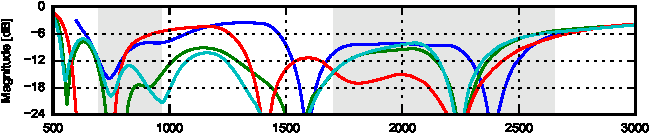
\includegraphics{img/soren/ue/design2sn/s11top.pdf}\\
        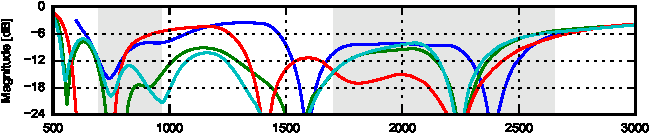
\includegraphics{img/soren/ue/design2sn/s11top.pdf}\\
        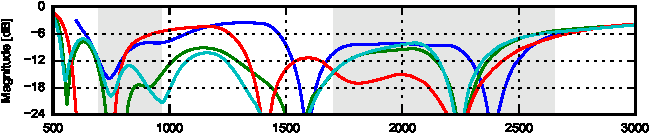
\includegraphics{img/soren/ue/design2sn/s11top.pdf}
    \end{center}
    \legendfooter
\end{frame}

\begin{frame}
    \frametitle{User Effects -- S22, minimum over tunable range}
    \begin{center}
        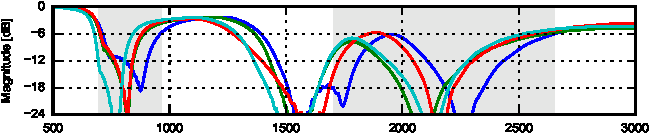
\includegraphics{img/soren/ue/design2sn/s22side.pdf}\\
        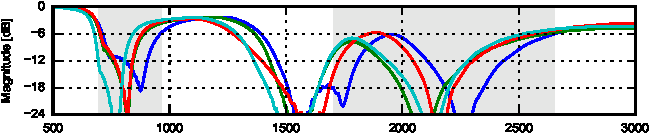
\includegraphics{img/soren/ue/design2sn/s22side.pdf}\\
        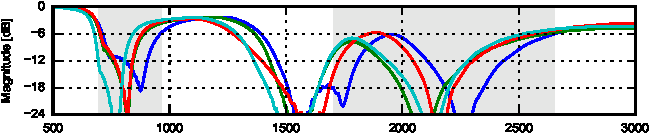
\includegraphics{img/soren/ue/design2sn/s22side.pdf}
    \end{center}
    \legendfooter
\end{frame}

% \begin{frame}
%     \frametitle{User Effects -- S21, minimum over tunable range (tuning top)}
%     \begin{center}
%         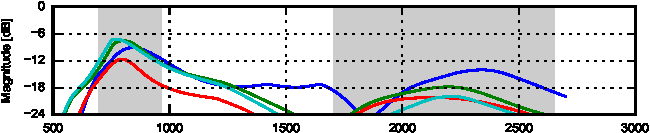
\includegraphics{img/soren/ue/design2sn/s21top.pdf}\\
%         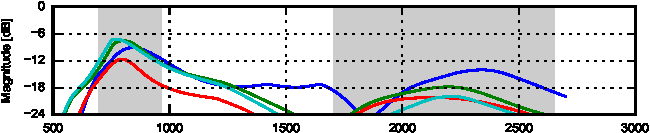
\includegraphics{img/soren/ue/design2sn/s21top.pdf}\\
%         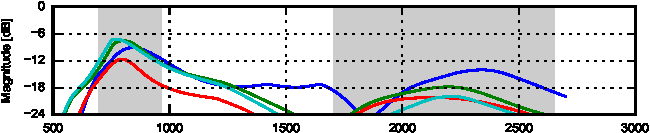
\includegraphics{img/soren/ue/design2sn/s21top.pdf}
%     \end{center}
%     \legendfooter
% \end{frame}
% 
% \begin{frame}
%     \frametitle{User Effects -- S21, minimum over tunable range (tuning side)}
%     \begin{center}
%         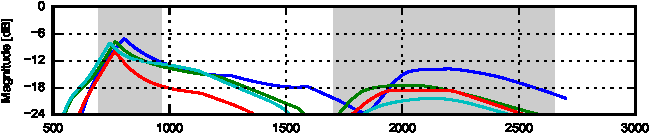
\includegraphics{img/soren/ue/design2sn/s21side.pdf}\\
%         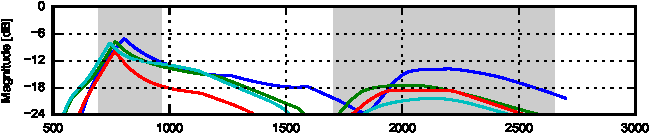
\includegraphics{img/soren/ue/design2sn/s21side.pdf}\\
%         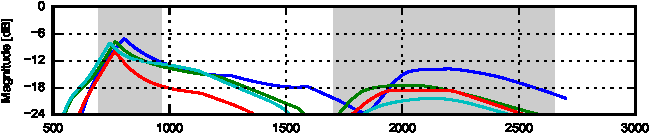
\includegraphics{img/soren/ue/design2sn/s21side.pdf}
%     \end{center}
%     \legendfooter
% \end{frame}

\begin{frame}
    \frametitle{User Effects -- Total efficiency, minimum over tunable range (top)}
    \begin{center}
        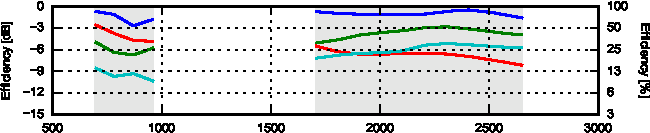
\includegraphics{img/soren/ue/design2sn/efftop.pdf}\\
        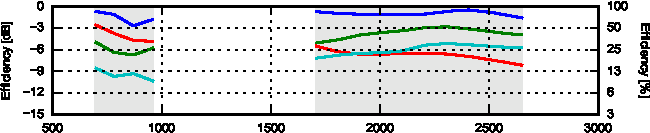
\includegraphics{img/soren/ue/design2sn/efftop.pdf}\\
        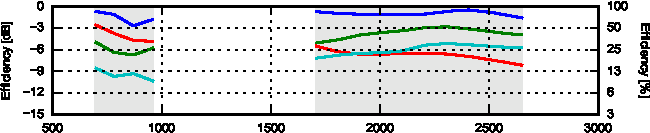
\includegraphics{img/soren/ue/design2sn/efftop.pdf}
    \end{center}
    \legendfooter
\end{frame}

\begin{frame}
    \frametitle{User Effects -- Total efficiency, minimum over tunable range (side)}
    \begin{center}
        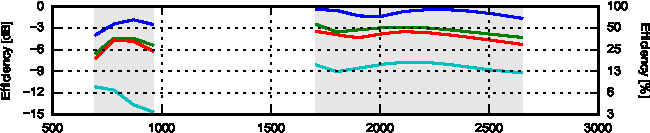
\includegraphics{img/soren/ue/design2sn/effside.pdf}\\
        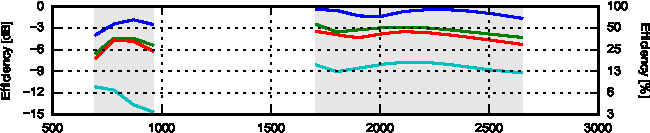
\includegraphics{img/soren/ue/design2sn/effside.pdf}\\
        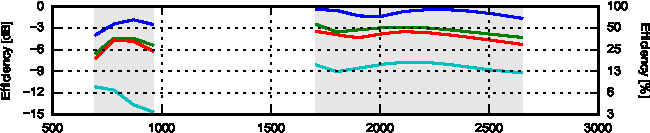
\includegraphics{img/soren/ue/design2sn/effside.pdf}
    \end{center}
    \legendfooter
\end{frame}

\begin{frame}
    \frametitle{User Effects -- Correlation, minimum over tunable range (top)}
    \begin{center}
        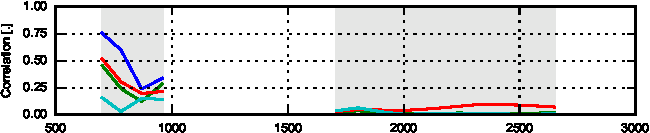
\includegraphics{img/soren/ue/design2sn/corrtop.pdf}\\
        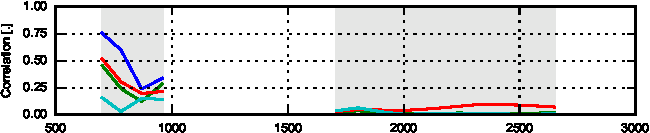
\includegraphics{img/soren/ue/design2sn/corrtop.pdf}\\
        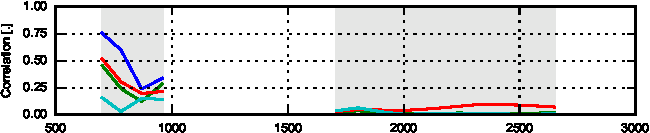
\includegraphics{img/soren/ue/design2sn/corrtop.pdf}
    \end{center}
    \legendfooter
\end{frame}

\begin{frame}
    \frametitle{User Effects -- Correlation, minimum over tunable range (side)}
    \begin{center}
        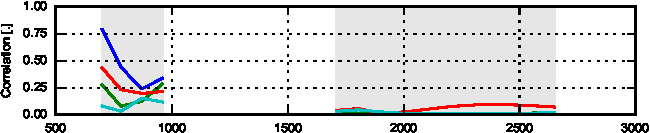
\includegraphics{img/soren/ue/design2sn/corrside.pdf}\\
        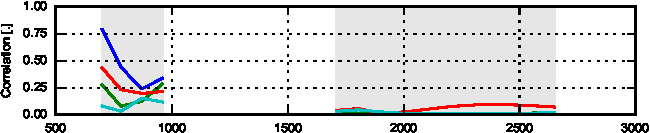
\includegraphics{img/soren/ue/design2sn/corrside.pdf}\\
        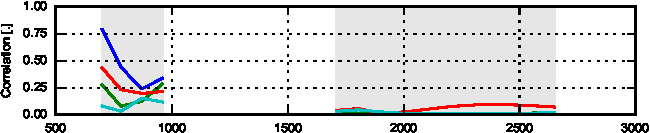
\includegraphics{img/soren/ue/design2sn/corrside.pdf}
    \end{center}
    \legendfooter
\end{frame}

\section{Prototypes}
\begin{frame}
    \frametitle{Prototypes}
\end{frame}

\begin{frame}
    \frametitle{Preliminary Conclusion}
\end{frame}
